For the scaling functions we find at this order:
\begin{align}
\bar c_{\tVA,xF_3,\Pq}^{(1),F} &= \bar c_{\tVA,g_4,\Pq}^{(1),F} = \bar c_{\tVA,g_L,\Pq}^{(1),F} = 0
\end{align}
and 
\begin{align}
\bar c_{\tVV,2xg_1,\Pq}^{(1),F} &= \bar c_{\tAA,2xg_1,\Pq}^{(1),F}
\end{align}
and furthermore near threshold, we find
\begin{align}
\bar c_{\vec k,\Pq}^{(1),F,\tThr} &= -c_{\vec k,\Pg}^{(0),\text{thr}} \frac{\beta^2\rho_q}{\pi^2(\rho_q-1)} \frac{K_{\Pq\Pgg}}{24K_{\Pg\Pgg}} \cdot \bar a_{\vec k,\Pq}^{(1,0)}
\end{align}
with
\begin{align}
\bar a^{(1,0)}_{\tVV,F_2,\Pq} &= 1\\
\bar a^{(1,0)}_{\tVV,F_L,\Pq} &= \bar a^{(1,0)}_{\tVV,F_2,\Pq} - \frac 2 {3}\\
\bar a^{(1,0)}_{\tVV,2xg_1,\Pq} &= \bar a^{(1,0)}_{\tAA,F_2,\Pq} = \bar a^{(1,0)}_{\tAA,F_L,\Pq} = \bar a^{(1,0)}_{\tAA,2xg_1,\Pq} = \bar a^{(1,0)}_{\tVV,F_2,\Pq}
\end{align}

\begin{figure}[ht!]
\centering
\begin{subfigure}[t]{.3\textwidth}
	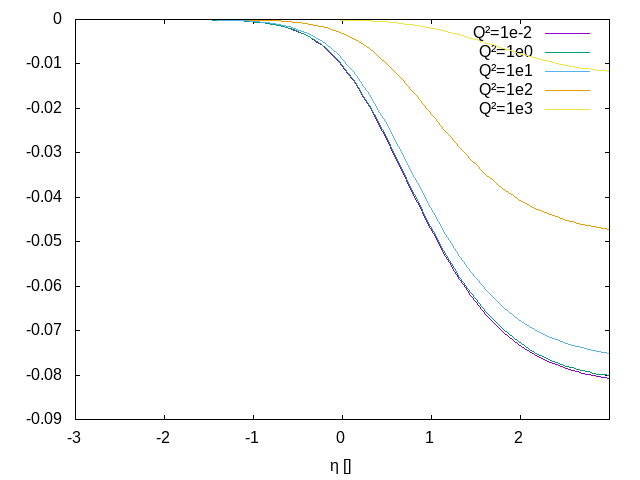
\includegraphics[width=\textwidth]{../../img2/partonic/cqBarF1_VV_F2}
\end{subfigure}%
\begin{subfigure}[t]{.3\textwidth}
	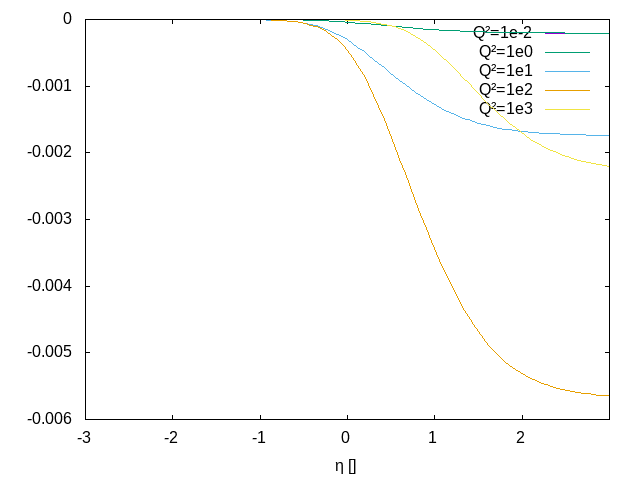
\includegraphics[width=\textwidth]{../../img2/partonic/cqBarF1_VV_FL}
\end{subfigure}%
\begin{subfigure}[t]{.3\textwidth}
	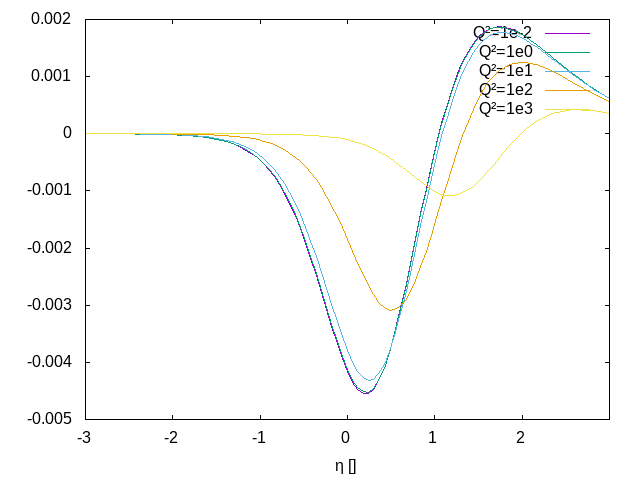
\includegraphics[width=\textwidth]{../../img2/partonic/cqBarF1_VV_x2g1}
\end{subfigure}\\%
\begin{subfigure}[t]{.3\textwidth}
	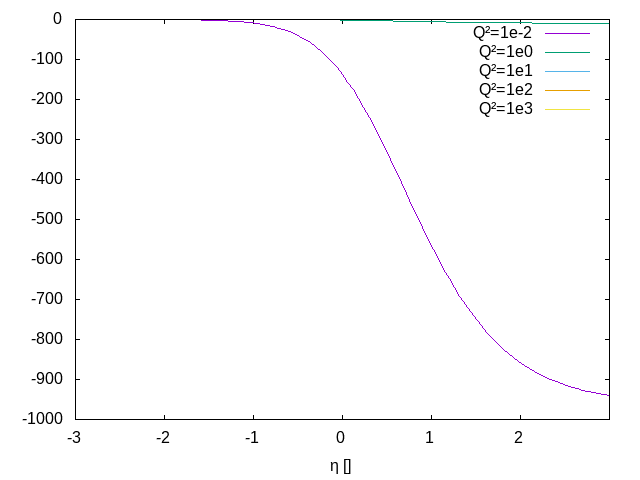
\includegraphics[width=\textwidth]{../../img2/partonic/cqBarF1_AA_F2}
\end{subfigure}%
\begin{subfigure}[t]{.3\textwidth}
	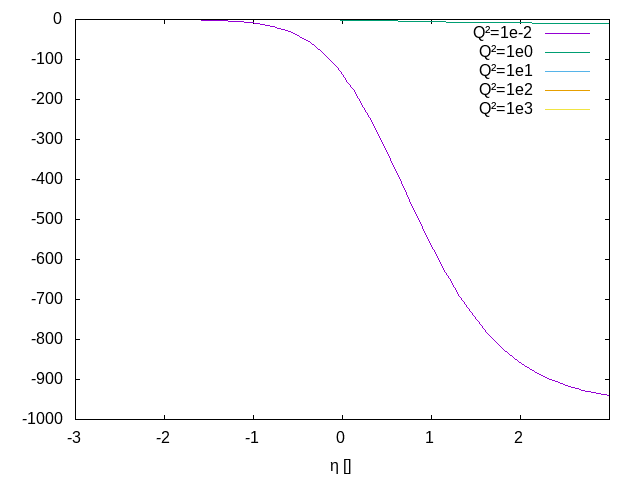
\includegraphics[width=\textwidth]{../../img2/partonic/cqBarF1_AA_FL}
\end{subfigure}%
\begin{subfigure}[t]{.3\textwidth}
	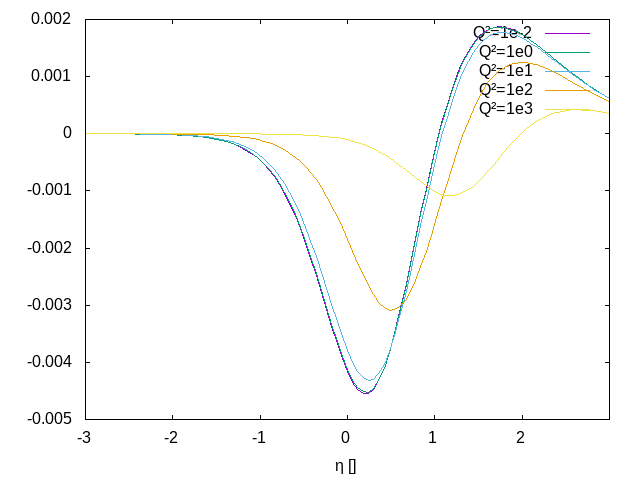
\includegraphics[width=\textwidth]{../../img2/partonic/cqBarF1_AA_x2g1}
\end{subfigure}%
\caption{next-to-leading order scaling functions $\bar c_{k,\Pq}^{(1),F}(\eta,\xi)$ plotted as function of $\eta=s/(4m^2)-1$ for different values of $Q^2$ in units of $\si{\GeV^2}$ at $m=\SI{4.75}{\GeV}$ (i.e. different values of $\xi=Q^2/m^2$) }\label{fig:cqBarF1}
\end{figure}
